\documentclass[a4paper, 12pt]{article}%тип документа

%отступы
\usepackage[left=2cm,right=2cm,top=2cm,bottom=3cm,bindingoffset=0cm]{geometry}

%Русский язык
\usepackage[T2A]{fontenc} %кодировка
\usepackage[utf8]{inputenc} %кодировка исходного кода
\usepackage[english,russian]{babel} %локализация и переносы

%Вставка картинок
\usepackage{wrapfig}
\usepackage{graphicx}
\graphicspath{{pictures/}}
\DeclareGraphicsExtensions{.pdf,.png,.jpg}

%оглавление
\usepackage{titlesec}
\titlespacing{\chapter}{0pt}{-30pt}{12pt}
\titlespacing{\section}{\parindent}{5mm}{5mm}
\titlespacing{\subsection}{\parindent}{5mm}{5mm}
\usepackage{setspace}

%Графики
\usepackage{multirow}
\usepackage{pgfplots}
\pgfplotsset{compat=1.9}

%Математика
\usepackage{amsmath, amsfonts, amssymb, amsthm, mathtools}

%Стиль страницы
\usepackage{fancyhdr}
\pagestyle{fancy}

\begin{document}

\begin{titlepage}

\begin{center}
%\vspace*{1cm}
\large\textbf{Московский Физико-Технический Институт}\\
\large\textbf{(государственный университет)}
\vfill
\line(1,0){430}\\[1mm]
\huge\textbf{Работа 19}\\
\line(1,0){430}\\[1mm]
\vfill
\large Сибгатуллин Булат, ФРКТ\\
\end{center}

\end{titlepage}
\fancyhead[L] {Работа 19}
\noindent \textbf{Цель работы:} \\
\indent Изучение работы методов активных фильтров.\\
\noindent \textbf{В работе используются:} \\
\indent Программа MicroCap10.

\section{Звенья первого порядка}

\begin{enumerate}

\item Откроем в Micro-Cap модель \textbf{zpole.cir} пропорционально интегрирующей и дифференцирующей цепей с полусом в точке $s =\frac{p}{\omega_0} = -1$, $f_0 = \frac{\omega_0}{2\pi}= 10k$ и нулями в точках $s = -2$ и $s = -\frac{1}{2}$. Измерим уровни подавления на частоте $f_0$ и в полосах задержания:

\[K_{f_0} = 0,79\]

\[\text{В полосах задержания}: K = 0,5\]

Оценим положения и уровни экстремумов фазовых характеристик:

\[\text{Дифференцирующая}: max = 19,5^{\circ}\]

\[\text{Интегрирующая}: min = -19,5^{\circ}\]

\item Изменим номиналы резисторов в схемах так, чтобы сохранив положения полюсов, переместить нули в точки $s = -4$, $s = -\frac{1}{4}$. Измерим уровни подавления на частоте $f_0$ и в полосах задержания:

\[K_{f_0} = 0,73\]

\[\text{В полосах задержания}: K = 0,25\]

Оценим положения и уровни экстремумов фазовых характеристик:

\[\text{Дифференцирующая}: max = 36,9^{\circ}\]

\[\text{Интегрирующая}: min = -36,9^{\circ}\]

\item Откроем модель $\textbf{integrator.cir}$ реального интегратора с частотой единичного усиления $f_1 = 10k$ и усилением $K = \frac{R_K}{R}$. Варьируя резистор $R_K = [20k, 640k|log2]$, изучим поведение нормированных частотных и фазовых характеристик:

\begin{figure}[h!]
\centering	
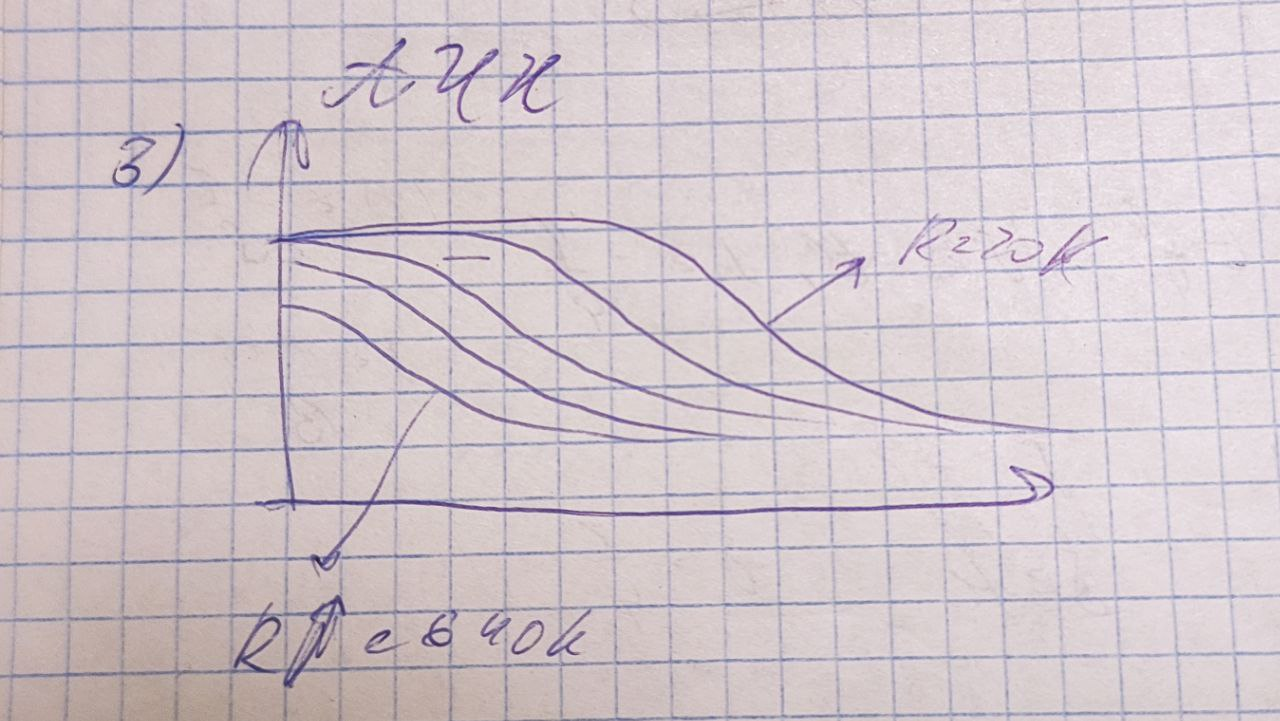
\includegraphics[width=0.7\textwidth]{images/1_3.jpg}
\caption{Аплитудно частотная характеристика}
\label{1_3}
\end{figure}

\item Подключив источник \textit{step} единичного интегратора $h_0(t / \tau_1)$, $\tau_1 = RC = 15.92\mu$, варьируя $R_K = [20k, 640k|log2]$. Оценим значения ошибок интегрирования в точках $\frac{t}{\tau_1} = \frac{K}{2}$:

\begin{center}
\begin{tabular}{|c|c|c|c|c|c|c|}
\hline 
$\sigma, \%$ & 18 & 19 & 19,5 & 19,7 & 20 & 20 \\ 
\hline 
$K$ & 2 & 4 & 8 & 16 & 32 & 64 \\ 
\hline 
\end{tabular} 
\end{center}

\end{enumerate}

\section{Активные звенья с двойным T-мостом}

\begin{enumerate}

\item Откроем модель полосового фильтра \textbf{pass2T.cir} с $f_0 = 10k, K_0 = 20$. Изучим его частотную и фазовую характеристики. Измерим усиление на частоте $f_0$ и полосу $\bigtriangleup f$ по уровню $-3dB$:

\[K = 7,5 \quad \bigtriangleup f = 1,9 \: \text{кГц}\]

Снимем зависимость усиления и ширины полосы от $R_2 = [20k, 100k|20k]$:

\begin{center}
\begin{tabular}{|c|c|c|c|c|c|}
\hline 
$R_2, k$ & 20 & 40 & 60 & 80 & 100 \\ 
\hline 
K & 7,5 & 14,6 & 21,8 & 28,9 & 36,1 \\ 
\hline 
\end{tabular} 
\end{center}

\item Изучим поведение фильтра при разбалансировании маста с варьированием $R_5 = [1.5k, 5.5k|500]$. Оценим значение $R_5$ при котором пиковое усиление достигает максимума:

\[R_5 = 3k\]

\item Изучим переходную характеристику фильтра. Измерим уровни скачка в нуле и первого выброса:

\[U_0 = 1 \: \text{В}\]

\[U_1 = 4,28 \: \text{В}\]

Прослежим за ее измением при варьировании $R_5 = [5.0k, 2.5k|500]$ и оценим значение $R_5$, при котором фильтр теряет устойчивость:

\[R_5 = 3k\]

\item Откроем модель режекторного фильтра \textbf{stop2T.cir} с $f_0 = 10k, \gamma = 0.1$. Изучим его частотную и фазовую характеристику. Измерить ширину полосы режекциии $\bigtriangleup f$ по уровню $-3 dB$:

\[\bigtriangleup f = 4 k\]

Изучим ее поведение при варьировании $R_1 = [90k, 240k|30k]$ и $R_1 = [300k, 1500k|300k]$:

\begin{figure}[h!]
\centering	
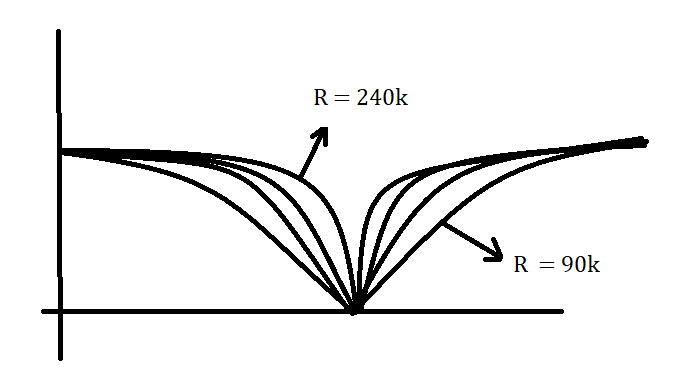
\includegraphics[width=0.7\textwidth]{images/2_4-1.png}
\caption{$R_1 = [90k, 240k|30k]$}
\label{2_4-1}
\end{figure}

\begin{figure}[h!]
\centering	
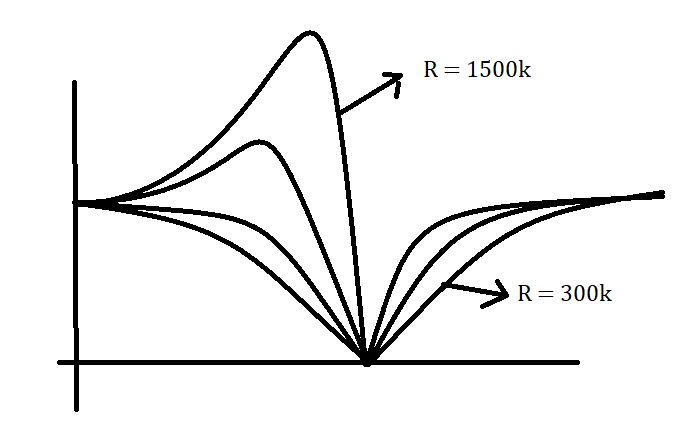
\includegraphics[width=0.7\textwidth]{images/2_4-2.png}
\caption{$R_1 = [300k, 1500k|300k]$}
\label{2_4-2}
\end{figure}

Изучим поведение фильтра при разбалансировании моста варьированием $R_5 = [1k, 9k|2k]$:

\begin{figure}[h!]
\centering	
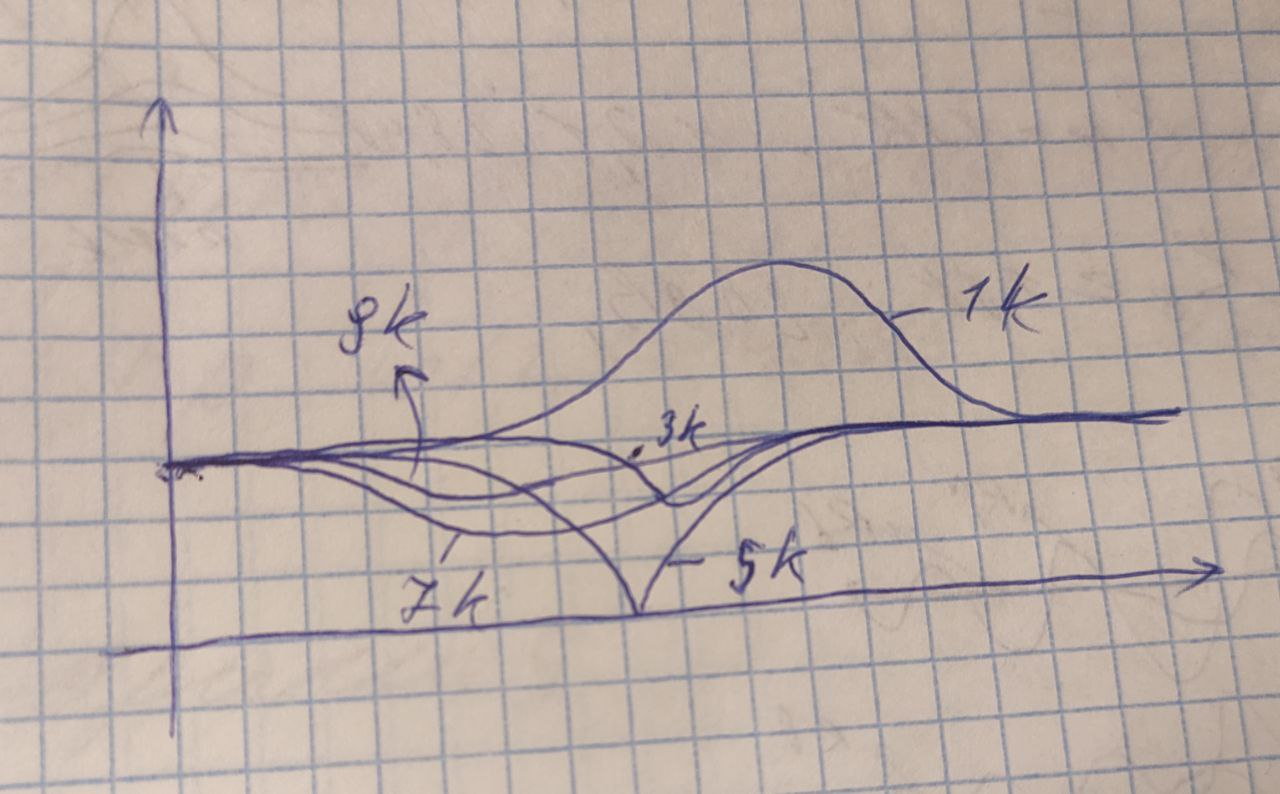
\includegraphics[width=0.7\textwidth]{images/2_5.jpg}
\caption{$R_5 = [1k, 9k|2k]$}
\label{2_5}
\end{figure}`

\item Изучим переходную характеристику фильтра. Измерим уровни скачка в нуле и первого выброса:

$U_0 = 1 \: \text{В}$

$U_1 = 0,7 \: \text{В}$

Проследим за ее изменением при варьировании $R_1 = [90k, 240k|30k]$ и $R_5 = [1k, 9k|2k]$:

\begin{figure}[h!]
\centering	
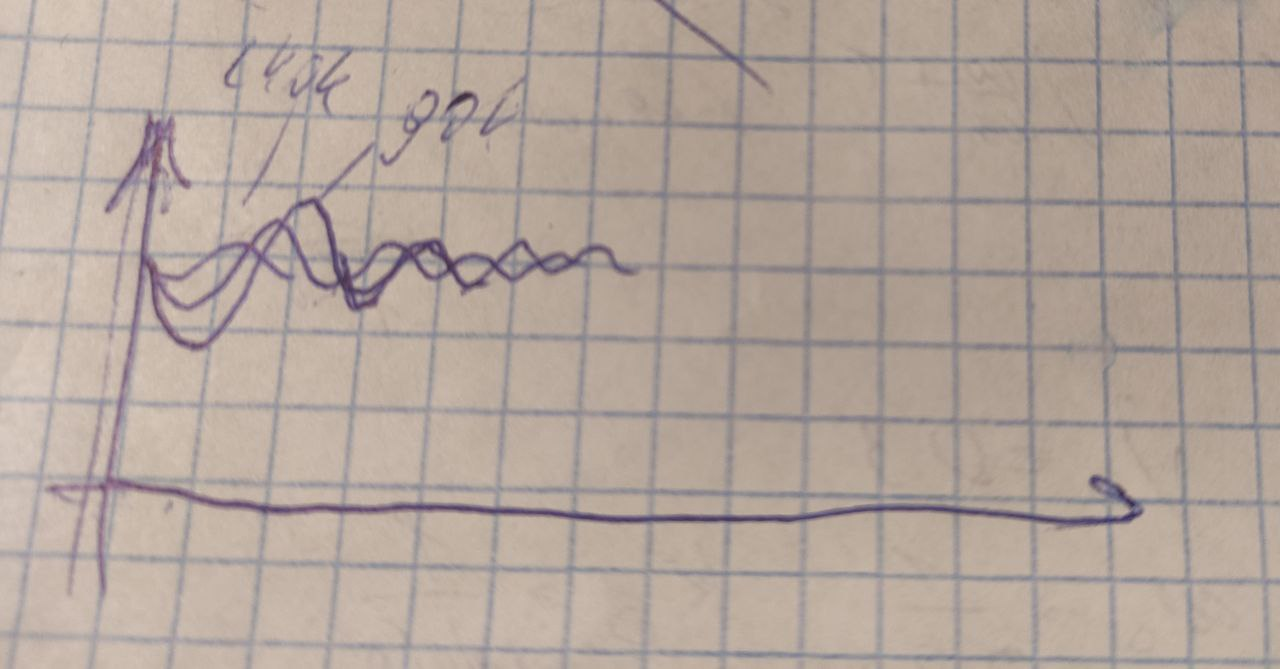
\includegraphics[width=0.7\textwidth]{images/2_5-1.jpg}
\caption{$R_1 = [90k, 240k|30k]$}
\label{2_5-1}
\end{figure}`

\begin{figure}[h!]
\centering	
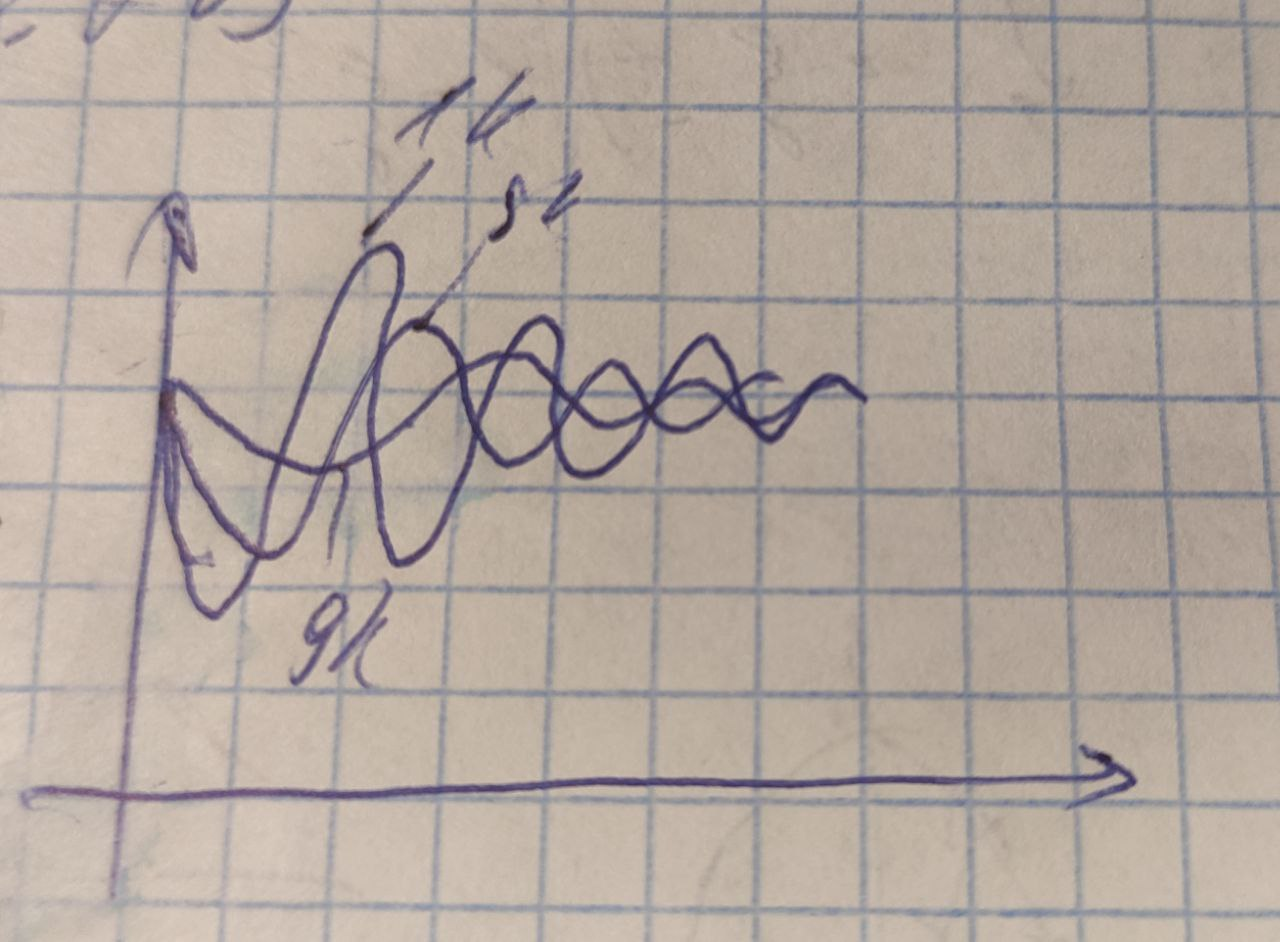
\includegraphics[width=0.7\textwidth]{images/2_5-2.jpg}
\caption{$R_5 = [1k, 9k|2k]$}
\label{2_5-2}
\end{figure}`

\end{enumerate}

\section{Звенья Саллена-Ки}

\begin{enumerate}

\item Откроем модель \textbf{skey.cir} звеньев Саллена-Ки с частотой $f_0 = 10k$ и добротностью $Q = 1$. Изучим частотные характеристики звеньев. Измерим значение коэффициентов передачи:

\[\textit{ФНЧ}: \quad K = 1\]
\[\textit{ФВЧ}: \quad K = 1\]
\[\textit{ПФ}: \quad K = 1\]

Проанализируем изменение частотных характеристик фильтров при варьировании резисторов $R_L, R_H, R_P = [11k, 19k|2k].$ %добавить графики было бы неплохо
 Измерим пиковые значения усиления при $R_{L,H,P} = 19k$:

\[\textit{ФНЧ}: \quad U = 29,4 \: \text{В}\]
\[\textit{ФВЧ}: \quad U = 28,4 \: \text{В}\]
\[\textit{ПФ}: \quad U = 28,8 \: \text{В}\]

\item Исследуем переходные характеристики фильтров и их поведение при варьировании $R_L, R_H, R_P = [11k, 19k|2k].$ %тут тоже нужны графики

\item Откроем модель $\textbf{sk3pole.cir}$ с фильтрами Баттерворта верхних и нижних частот порядка n = 3 на частоту среза $f_0 = 10k$. Проанализируем частотные характеристики фильтров. Измерим скорость спада в $dB$ на октаву и затухания на частотах $f_0 / 2, 2f_0$:

\[\textit{ФНЧ}: \quad 2f_0 \rightarrow -18 dB\]
\[textit{ФВЧ}: \quad f_0 / 2 \rightarrow -18 dB\]

Преобразуем их в фильтры Чебышева с $\varepsilon = 1$. Параметры полюсов ФНЧ можно получить в $MatLab$ командой highpass(cheb(3,1)). Измерим уровни затухания на частотах $f_0 / 2, 2f_0$ и $F_0 / 10, 10f_0$:

\[textit{ФНЧ}: \quad 2f_0 \rightarrow -26 dB, \: 10f_0 \rightarrow -69 dB\]
\[\textit{ФВЧ}: \quad f_0 / 2 \rightarrow -26 dB, \: f_0 / 10 \rightarrow -69 dB\]

\item Открыв прототип \textbf{sk4pole.cir} реализуем 4-полюсной полосовой фильтр Чебышева с $f_0 = 10k, \varepsilon = 1, Q = \frac{f_0}{\bigtriangleup f} = 6$. Измерим уровни затухания на частотах $f_0 / 2, 2f_0$ и $F_0 / 10, 10f_0$:

\[textit{ФНЧ}: \quad 2f_0 \rightarrow -41 dB, \: 10f_0 \rightarrow -73,8 dB\]
\[\textit{ФВЧ}: \quad f_0 / 2 \rightarrow -41 dB, \: f_0 / 10 \rightarrow -73,8 dB\]

\end{enumerate}

\section{Звенья с двойной обратной связью}

\begin{enumerate}

\item Откроем прототип \textbf{amp1bp.cir} и реализуем полосовое звено с $f_0 = 5k, K_0 = 5, Q = 15$. Измерим ширину полосы по уровню 0.7 = -3dB и пиковое усиление $QK_0$, оценим добротность:

\[\bigtriangleup f = 0.35k\]
\[Q \simeq 14.3\]
\[QK_0 \simeq 75\]

Изучить поведение АЧХ при варьировании $R_2 = [100, 1.3k|200]$. Построить график зависимости частоты пика от $R_2$.

\begin{center}
\begin{tabular}{|c|c|c|c|c|c|c|c|}
\hline 
$f, \: \text{кГц}$ & 4,11 & 4,38 & 4,74 & 5,27 & 6,18 & 7,65 & 12,7 \\ 
\hline 
$R, \: \text{кОм}$ & 1,3 & 1,1 & 0,9 & 0,7 & 0,5 & 0,3 & 0,1 \\ 
\hline 
\end{tabular} 
\end{center}

\begin{figure}[h!]
\centering	
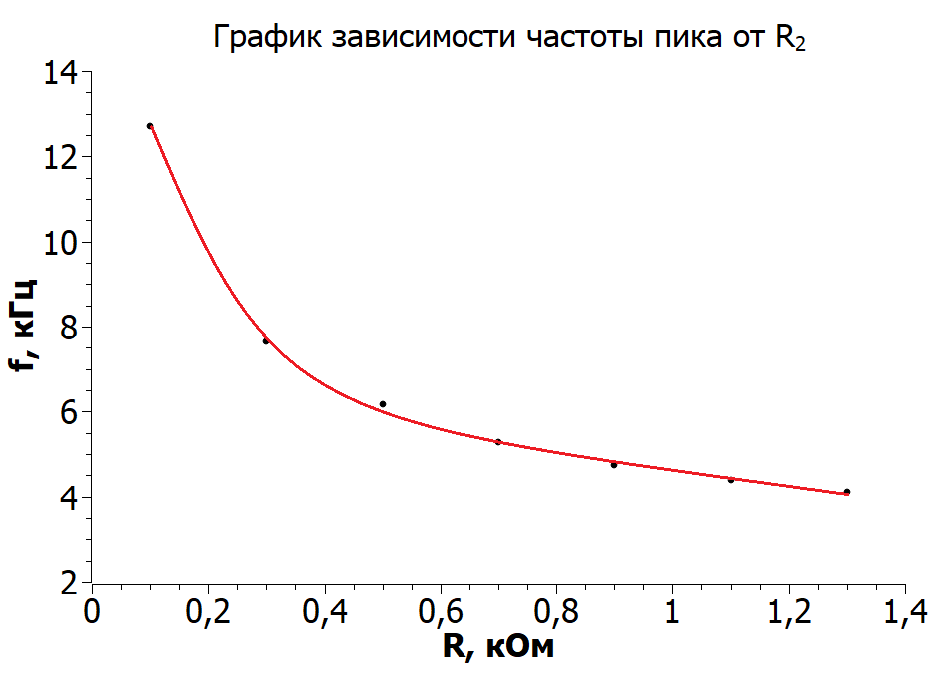
\includegraphics[width=0.7\textwidth]{images/5_1.png}
\caption{$R_2 = [100, 1.3k|200]$}
\label{2_5-2}
\end{figure}`

\item Соберем звено на макетной плате. Экспериментально измерим параметры $K_0, f_0, Q$:

\[f_0 = 5,5 \: \text{кГц}\]

\[K_0 = 62,5\]

\[\bigtriangleup f = 0,48\]

\[Q \simeq 11,45\]

\[K_0 \simeq 5,46\]

Также можем заметить совпадение переходных характеристик собранной и смоделированной схемы.

\item Откроем прототип \textbf{cheb6pole.cir} и реализуем шестиполюсный полосовой фильтр Чебышева с параметрами $f_0 = 1k, \varepsilon = 1, Q = 3$. Измерим затухания на частотах $0.1k,0.5k, 2k, 10k$:

\[f = 100: \: 100 dB\]
\[f = 500: \: 51 dB\]
\[f = 2k: \: 51.5 dB\]
\[f = 10k: \: 101 dB\]

\end{enumerate}

\section{Звенья эллиптических фильтров}

\begin{enumerate}

\item Выберем параметр селективности $\eta = 1,3$. Реализуем трехполюсной элликптический фильтр нижних частот с параметрами $f_0 = 1k, \varepsilon = 1, \eta = 1,3$. Изучим частотную характеристику фильтра и частотные характеристики составляющих его звеньев. По фазовой характеристике установим, что нуль находится в правой полуплоскости. Определим уровень затухания и границу полосы задержания:

\[\eta_1 = 25,6 dB\]

\[\eta \simeq 3 dB\]

\end{enumerate}

\end{document}